% Template for a Computer Science Tripos Part II project dissertation
\documentclass[12pt,a4paper,twoside,openright]{report}
\usepackage[pdfborder={0 0 0}]{hyperref}    % turns references into hyperlinks
\usepackage[margin=25mm]{geometry}  % adjusts page layout
\usepackage{graphicx}  % allows inclusion of PDF, PNG and JPG images
\usepackage{verbatim}
\usepackage{docmute}   % only needed to allow inclusion of proposal.tex
\usepackage{fancyvrb}
\usepackage{color}


\DefineVerbatimEnvironment{blockcode}
  {Verbatim}
  {fontsize=\small}

\raggedbottom                           % try to avoid widows and orphans
\sloppy
\clubpenalty1000%
\widowpenalty1000%

\renewcommand{\baselinestretch}{1.1}    % adjust line spacing to make
                                        % more readable

\begin{document}

\bibliographystyle{plain}


%%%%%%%%%%%%%%%%%%%%%%%%%%%%%%%%%%%%%%%%%%%%%%%%%%%%%%%%%%%%%%%%%%%%%%%%
% Title


\pagestyle{empty}

\rightline{\LARGE \textbf{George Ash}}

\vspace*{60mm}
\begin{center}
\Huge
\textbf{} \\[5mm]
Computer Science Tripos -- Part II \\[5mm]
Fitzwilliam College \\[5mm]
\today  % today's date
\end{center}

%%%%%%%%%%%%%%%%%%%%%%%%%%%%%%%%%%%%%%%%%%%%%%%%%%%%%%%%%%%%%%%%%%%%%%%%%%%%%%
% Proforma, table of contents and list of figures

\pagestyle{plain}

\chapter*{Proforma}

{\large
\begin{tabular}{ll}
Name:               & \bf George Ash                       \\
College:            & \bf Fitzwilliam College                     \\
Project Title:      & \bf Smart Antialiasing for Consumer Virtual Reality \\
Examination:        & \bf Computer Science Tripos -- Part II, July 2017  \\
Word Count:         & \bf 1587\footnotemark[1] \\
Supervisor:         & Dr Rafal Mantiuk                    \\ 
\end{tabular}
}
\footnotetext[1]{This word count was computed
by \texttt{detex diss.tex | tr -cd '0-9A-Za-z $\tt\backslash$n' | wc -w}
}
\stepcounter{footnote}


\section*{Original Aims of the Project}

To examine the effect on the image quality and GPU load when applying antialiasing only to a small field of view in a consumer Virtual Reality (VR) Headmounted Display (HMD).


\section*{Work Completed}

Implementation of a generic, seamless method to multisample only in the centre of the screen using OpenGL. Examined an implementation to accomodate to Foveated Rendering.
A user study was conducted that determined image quality across a range of antialiasing techniques.

\section*{Special Difficulties}

Learning to profile accurately GPU software.
Learning OpenGL in depth.
 
\newpage
\section*{Declaration}

I, [Name] of [College], being a candidate for Part II of the Computer
Science Tripos [or the Diploma in Computer Science], hereby declare
that this dissertation and the work described in it are my own work,
unaided except as may be specified below, and that the dissertation
does not contain material that has already been used to any substantial
extent for a comparable purpose.

\bigskip
\leftline{Signed [signature]}

\medskip
\leftline{Date [date]}

\tableofcontents

\listoffigures

\newpage
\section*{Acknowledgements}

This document owes much to an earlier version written by Simon Moore
\cite{Moore95}.  His help, encouragement and advice was greatly 
appreciated.

%%%%%%%%%%%%%%%%%%%%%%%%%%%%%%%%%%%%%%%%%%%%%%%%%%%%%%%%%%%%%%%%%%%%%%%
% now for the chapters

\pagestyle{headings}

\chapter{Introduction}

\section{Background}

Through the affordability of display panels and cheap wide-angle lenses, Virtual Reality Displays are beggining to flood the consumer market. To meet this demand, efficient rendering software and practices will need to be adopted.

Graphics rendering pipelines take good advantage of available GPU power. But the constraints of realistic, immersive virtual reality present a huge challenge to engineers. They must output a high resolution, wide field of view, antialiased image, with a response to stimulus time under 20ms.

As this technology progresses and matures, it will become increasingly important to provide low-latency response times. Resolutions will need to increase to around 8K*8K, but to achieve this our graphics processing hardware and software will have to evolve too.

Aliasing in graphics refers to spatial and temporal artefacts present in a rendered image. They are the result of sampling a higher frequency signal component at a lower freqency.

Antialising is the process of removing such artefacts, but this has to be done efficiently or we will sacrifice frame drops and potential motion sickness for the end-user.
There are a multitude of antialiasing approaches, though most sample at a higher frequency than will be presented in the final image, then downsampling through some filter. 


\section{Common Antialiasing Approaches}

There are a multitude of antialising approaches, one of the most common is Supersampled Anti-alising (SSAA).
First the scene is sampled at an integer multiple higher resolution than we intend to present it.
Then, before presenting, this image is downsampled by taking for each pixel in the presented image, a linear combination of its closest neighbors in the higher resolution image. In the figure below, to calculate the final pixels colour, 4 samples per pixel are computed, each run through the fragment shader and then these pixels each contribute to the resulting image. The formula for for determining the final colour of the pixel is the simple mean average for each colour (Red, Green and Blue):
$$ c = \frac{1}{n}\displaystyle\sum_{i=1}^n c_i $$ where n is the number of samples per pixels we take.



\begin{figure}
\setlength{\unitlength}{1mm}-
\begin{center}
\begin{picture}(125,100)

\put(10,65){High-res image}

\put(0,40){\framebox(20,20){$1_1$}}
\put(20,40){\framebox(20,20){$1_2$}}
\put(0,20){\framebox(20,20){$1_3$}}
\put(20,20){\framebox(20,20){$1_4$}}

\put(40,55){\vector(1,0){20}}
\put(40,45){\vector(1,0){20}}
\put(40,25){\vector(1,0){20}}
\put(40,35){\vector(1,0){20}}

\put(50,75){Fragment Shader}
\put(60,10){\framebox(10,60)}

\put(70,33){\vector(1,0){20}}
\put(70,38){\vector(1,0){20}}
\put(70,43){\vector(1,0){20}}
\put(70,48){\vector(1,0){20}}

\put(88,55){Presented Image}
\put(90,30){\framebox(20,20){1}}



\end{picture}
\end{center}
\caption{An example of 4x Supersampling for a single pixel.}
\label{latexpic1}
\end{figure}

Another common approach, that is built into the OpenGL API, is Multisampled Anti-aliasing (MSAA). As before, the scene is sampled at a higher resolution than we intend to present it. If one of the subsamples is covered by a triangle being rendered, a fragment shader must be run on the whole sample, but the result of that fragment shader is applied to all subsamples. This means that fragment shader only has to be run the same number of times as it would have in the single sampled image. 
MSAA provides a significant speedup over SSAA and is widely employed in practice, but only removes spatial artefacts at polygon edges. SSAA can remove artefacts within polygons, an example of which will be presented later.

\section{Virtual Reality Headmounted Displays}

A typical virtual Reality Headmounted Display (HMD) is comprised of 2 main components: The screen - to which our rendered image is presented and a wide-angle lens - to project the displayed image into the eye. The lens allows for the user to focus on a screen that is normally too close for the eye to focus on by itself. 
Side effects of the lens used in the Oculus Rift DK2 are chromatic abberation, pincushion distortion, and astigmatism.\\

Chromatic abberation refers to the separation of colour due to the different refractive indexes for different wavelengths of light. A Virtual Reality API should correct for this.\\

Pincushion distortion refers to the stretching of the image near the egdes. The inverse of pincushion distortion, barrel disortion, can be applied to reverse the effects of pincushion distortion. The barrel distortion that we apply results in a varying number of texels per pixel in our final image, a property will be explored in the second extension. Again a Virtual Reality API should apply barrel distortion for you.


\begin{figure}[tbh]
\centerline{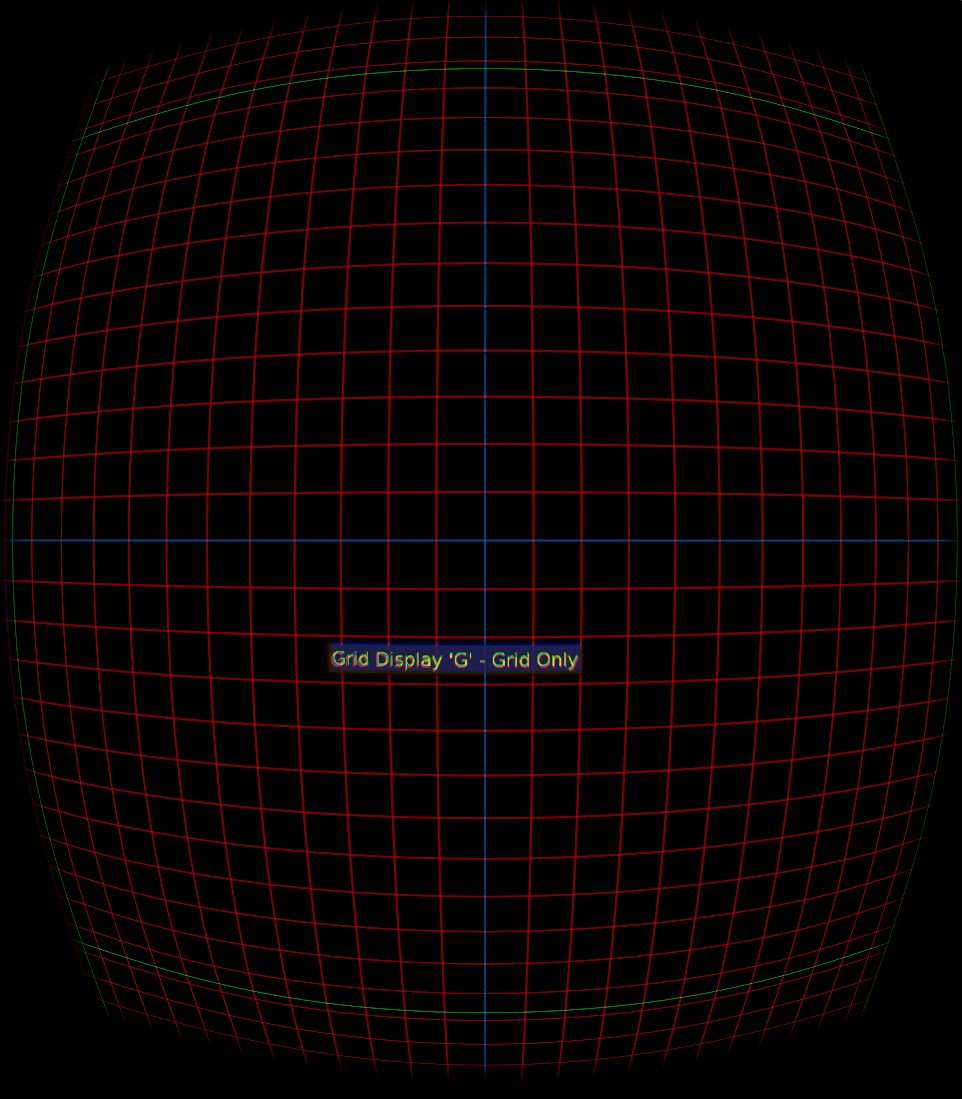
\includegraphics[width=10cm]{figs/distortiongrid.png}}
\caption{Barrel distortion applied to a rectangular grid}
\label{distortiongrid}
\end{figure}

Lens astigmatism is a property of the lenses used in most consumer HMDs. Because of the astigmatism, the image presented to the user is sharp in the center but becomes progressivelly blurrier as you look towards the edges.  It can be corrected for by adding more lenses to the HMD, but this ends up being too expensive and bulky for consumer versions.

\begin{figure}
\centerline{
\includegraphics[width=8cm]{figs/blur.png}}
\caption{A depiction of lens astigmatism. The percieved image blurs as you move away from the sharp center.}
\label{blurred}
\end{figure}

This property can be exploited by antialiasing only where the image is sharpest, in the center. Graphical artefacts at the edges should be blurred enough to be unnoticable.



\chapter{Preparation}

This chapter outlines any preparatory work that was done before implementation of the two antialiasing approaches.

\section{OpenGL}

The OpenGL API provides an interface to render 3D graphics. It's oldest and most widely adopted open source API and provides some antialising functionality.

Some OpenGL terminology that will be used lots later.


\begin{description}

\item\texttt{Framebuffer} \\
  A collection of buffers that can be used as the destination for rendering.

\item\texttt{Blitting} \\
  The process of moving image data between framebuffers.

\item\texttt{Front Buffer}
  The buffer containing the image that is presented onscreen now. This buffer is contained within the Default Framebuffer.

\item\texttt{Back Buffer} \\
  The buffer containing the image that will be presented onscreen in the next frame, is contained within the Default Framebuffer. 

\item\texttt{Fragment} \\
  Collection of values produced by the rasterizer. A fragment represents a sample-sized segment of a rasterized primitive. These are processed by the fragment shader. 
\end{description}

\subsection{The OpenGL pipeline}

OpenGL provides a pipeline through which data about the rendered scene is processed and rasterized. A simplified view of it is presented here, given that some stages are optional or non-programmable.


\begin{figure}
\setlength{\unitlength}{0.8mm}-
\begin{center}
\begin{picture}(80,120)

\put(0,100){\framebox(80,10){Vertex Data}}
\put(0,80){\framebox(80,10){Vertex Shader}}
\put(0,60){\framebox(80,10){Geometry Shader}}
\put(0,40){\framebox(80,10){Primitive Assembly \& Rasterization}}
\put(0,20){\framebox(80,10){Fragment Shader}}
\put(0,0){\framebox(80,10){Per Sample Operations}}



\put(40,20){\vector(0,-1){10}}
\put(40,40){\vector(0,-1){10}}
\put(40,60){\vector(0,-1){10}}
\put(40,80){\vector(0,-1){10}}
\put(40,100){\vector(0,-1){10}}




\end{picture}
\end{center}
\caption{A glimpse at the OpenGL rendering pipeline}
\label{latexpic2}
\end{figure}

The Vertex Shader is run for every vertex in the scene. In the typical case it transforms vertexes in 3d world space to window space coordinates.

The Geometry Shader is run for every primitive in the scene (in all uses we'll simplify these to triangles). It is an unusual stage in that it can output more primitives than it takes as input. This stage is optional and can incur a heavy cost if utilized.

The Fragment shader is run for every fragment in the window space.

\section{Development}

Being relatively new to OpenGL I decided to build a small renderer to teach myself the basics of the API.

This small renderer proved invaluable to the success of the project, since I knew and understood the source code completely, I could implement and test an idea for optimisation or an implementation strategy quickly.

To get an idea of how these implementations would fare in a larger, more computationally intensive renderer I decided to modify the demo provided with the Oculus SDK 5.0.1: OculusWorldDemo.
The codebase to this was in C++ and the rendering code was written to be extensible - allowing for different graphics APIs to implement lower level rendering calls. The OpenGL implementation was Open Source and under the Apache License.

An agile approach was taken when implementing the antialising methods, stories were broken up into small, managable chunks. After these were implemented - extensions could be written up and implemented on top.
Due to the high degree of coupling between modules in the Demo, unit tests were deemed to time-consuming to write, and would have required extensive mocking of complex modules.
To make up for this, and to ensure correctness, runtime assertions were made on all branches and method calls.

\section{Software libraries}

The OculusVR SDK was used in the Demo to interface with the Oculus Rift DK2 HMD. An outdated version 0.5.0.1 was used being the last version to support linux.
The SDK provided vector and matrix math modules, runtime assertions, and allowed barrel distortion and chromatic abberation to be performed on colour buffers.

GLFW was used for context creation in the toy renderer.
GLM was used for matrix math in the toy renderer.

\section{Programming Languages}

C++ was used in both the toy renderer and OculusWorldDemo. It has native OpenGL bindings and has extensive compiler support allowing for performance to be maximised.


GLSL is the OpenGL C-like shader language that is run on the GPU. It was used to implement the first and second extensions. It's syntax is very similar to C. So learning it didn't take long.


\section{Development Tools}

Sublime text was the editor used to write all the software here.

The C/C++ debugger \texttt{gdb} was used to debug both the toy renderer and OculusWorldDemo

\texttt{apitrace} and \texttt{bugle} were used to debug and profile the OpenGL calls in both the toy renderer and OculusWorldDemo.

\subsection{Version Control}

Git was used as a version control system due to its flexibility and my familiarity with it. Remote repositories were placed both on a separate harddrive and Github. These remotes were updated on every commit. Commits were made after every development story was completed.

\subsection{Failsafes}

In the event of failure of my development machine, MCS machines were compatible and tested with the software I was using. Also two backups were made of all changes to the codebase, detailed above.

\chapter{Implementation}

\section{OculusWorldDemo Structure}

Given that the implementation of two antialiasing techniques is built on top of Oculus' existing work, it was first neccesary to understand a large portion of their codebase.
Here I give a brief overview of system components that will be modified and used later on. I also give a brief overview of Oculus' SDK before detailing components that were added and modified to OculusWorldDemo.


\section{Projection Transformation}

An essential component to 3D graphics is the projection transformation. It takes as input 3D coordinates and maps them to 2D window coordinates.
2 types of projection must be dealt with in the implementation.

\subsection{Orthographic projection}
The orthographic projection.
\[
 \begin{pmatrix}
  \frac{2}{right-left} & 0 & 0 & -\frac{right+left}{right-left} \\
  0 & \frac{2}{top-bottom} & 0 & -\frac{top+bottom}{right-left} \\
  0 & 0 & \frac{2}{far-near} & -\frac{far + near}{far-near} \\
  0 & 0 & 0 & 1
 \end{pmatrix}

This matrix is used to render two dimensional information at a required distance from the user.
\]
\subsection{Perspective projection}

The perspective 
\[
 \begin{pmatrix}
  a & b & c \\
  d & e & f \\
  g & h & i
 \end{pmatrix}
\]

\section{MultiSample Resolve}

This function takes as arguments a multisampled or supersampled texture along with an output texture. It then resolves the samples from the source texture to the target texture.


\begin{blockcode}[commandchars=\\\{\}, numbers=left]
void RenderDevice::ResolveMsaa(OVR::Render::Texture* msaaTex, OVR::Render::Texture* outputTex, float ratio)
\{
    bool isMsaaTarget = msaaTex->GetSamples() > 1;
    glBindFramebuffer( GL_READ_FRAMEBUFFER, MsaaFbo);
    glFramebufferTexture2D( GL_READ_FRAMEBUFFER, GL_COLOR_ATTACHMENT0,
                            isMsaaTarget ? GL_TEXTURE_2D_MULTISAMPLE : GL_TEXTURE_2D,
                            ((Texture*)msaaTex)->TexId, 0);
    glFramebufferRenderbuffer(GL_READ_FRAMEBUFFER, GL_DEPTH_ATTACHMENT, GL_RENDERBUFFER, 0);
    OVR_ASSERT(glCheckFramebufferStatus(GL_READ_FRAMEBUFFER) == GL_FRAMEBUFFER_COMPLETE);

    glBindFramebuffer( GL_DRAW_FRAMEBUFFER, CurrentFbo );
    glFramebufferTexture2D(GL_DRAW_FRAMEBUFFER, GL_COLOR_ATTACHMENT0, GL_TEXTURE_2D, ((Texture*)outputTex)->TexId, 0);
    glFramebufferRenderbuffer(GL_DRAW_FRAMEBUFFER, GL_DEPTH_ATTACHMENT, GL_RENDERBUFFER, 0);

    OVR_ASSERT(glCheckFramebufferStatus(GL_DRAW_FRAMEBUFFER) == GL_FRAMEBUFFER_COMPLETE);

\color{green}    int off_x = (outputTex->GetWidth() - outputTex->GetWidth()/ratio)/2; //Offset from bottom left of the target texture we wish to blit the source to. 
\color{green}    int off_y = (outputTex->GetHeight() - outputTex->GetHeight()/ratio)/2; // ditto
\color{green}    glBlitFramebuffer( 0, 0, msaaTex->GetWidth(), msaaTex->GetHeight(), off_x, off_y,
\color{green}                             off_x + outputTex->GetWidth()/ ratio,
\color{green}                             off_y + outputTex->GetHeight()/ ratio,
\color{green}                             GL_COLOR_BUFFER_BIT, GL_LINEAR);

    glBindFramebuffer( GL_FRAMEBUFFER, 0 );  
    GLint err = glGetError();
    OVR_ASSERT_AND_UNUSED(!err, err);
\}
\end{blockcode}

The method needs to set up the OpenGL state machine for the \texttt{glBlitFramebuffer} on line 21. First a multisampled framebuffer is set up to be read in line 2. Next we associate this framebuffer with \texttt{msaaTex} in lines 3-4. 
We then set up the destination texture in its own framebuffer, and set the GL state to draw to this buffer in the blit in lines 11-13.

Note that assertions are made to check for framebuffer completetness /*TODO*/define.

Lines 19-24 implement the last stage of the downsampling method given in Y. We only blit the color buffer and do a linear downsample. 

The GL_LINEAR filter will perform a supersample resolve using the method given in section BRAH.


\section{Tables}

\begin{samepage}
Here is a simple example\footnote{A footnote} of a table.

\begin{center}
\begin{tabular}{l|c|r}
Left      & Centred & Right \\
Justified &         & Justified \\[3mm]
%\hline\\%[-2mm]
First     & A       & XXX \\
Second    & AA      & XX  \\
Last      & AAA     & X   \\
\end{tabular}
\end{center}

\noindent
There is another example table in the proforma.
\end{samepage}

\section{Adding more complicated graphics}

The use of \LaTeX\ format can be tedious and it is often better to use
encapsulated postscript (EPS) or PDF to represent complicated graphics.
Figure~\ref{epsfig} and~\ref{xfig} on page \pageref{xfig} are
examples. The second figure was drawn using \texttt{xfig} and exported in
{\tt.eps} format. This is my recommended way of drawing all diagrams.


\begin{figure}[tbh]
\centerline{
\includegraphics{figs/cuarms.pdf}}
\caption{Example figure using encapsulated postscript}
\label{epsfig}
\end{figure}

\begin{figure}[tbh]
\vspace{4in}
\caption{Example figure where a picture can be pasted in}
\label{pastedfig}
\end{figure}


\begin{figure}[tbh]
\centerline{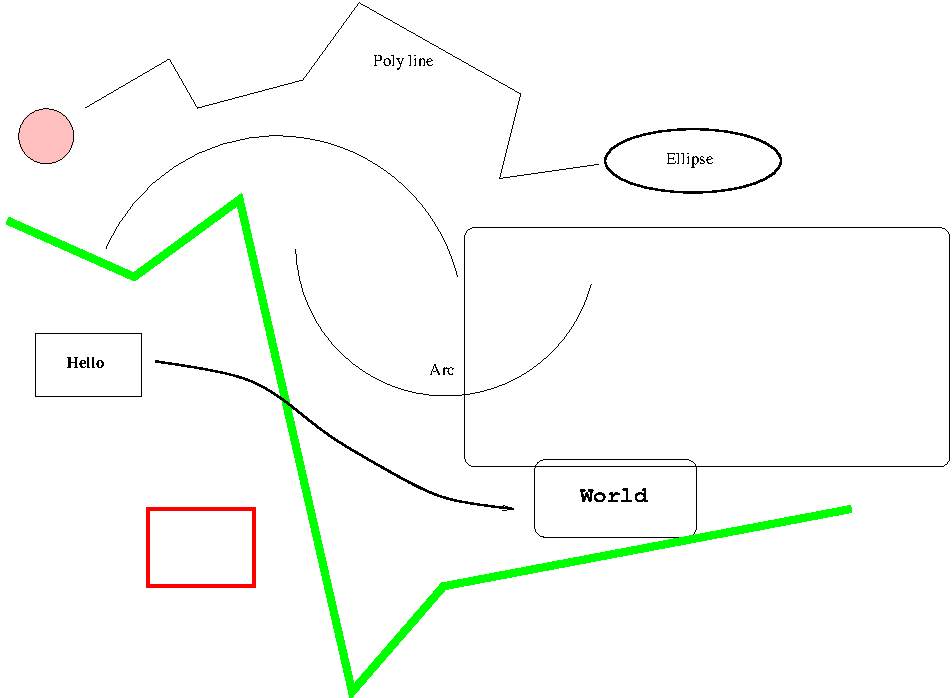
\includegraphics{figs/diagram.pdf}}
\caption{Example diagram drawn using \texttt{xfig}}
\label{xfig}
\end{figure}


\chapter{Evaluation}

\section{Printing and binding}

Use a ``duplex'' laser printer that can print on both sides to print
two copies of your dissertation. Then bind them, for example using the
comb binder in the Computer Laboratory Library.

\section{Further information}

See the Unix Tools notes at

\url{http://www.cl.cam.ac.uk/teaching/current-1/UnixTools/materials.html}


\chapter{Conclusion}

I hope that this rough guide to writing a dissertation is \LaTeX\ has
been helpful and saved you time.


%%%%%%%%%%%%%%%%%%%%%%%%%%%%%%%%%%%%%%%%%%%%%%%%%%%%%%%%%%%%%%%%%%%%%
% the bibliography
\addcontentsline{toc}{chapter}{Bibliography}
\bibliography{refs}

%%%%%%%%%%%%%%%%%%%%%%%%%%%%%%%%%%%%%%%%%%%%%%%%%%%%%%%%%%%%%%%%%%%%%
% the appendices
\appendix

\chapter{Latex source}

\section{diss.tex}
{\scriptsize\verbatiminput{diss.tex}}

\section{proposal.tex}
{\scriptsize\verbatiminput{proposal.tex}}

\chapter{Makefile}

\section{makefile}\label{makefile}
{\scriptsize\verbatiminput{makefile.txt}}

\section{refs.bib}
{\scriptsize\verbatiminput{refs.bib}}


\chapter{Project Proposal}

% Note: this file can be compiled on its own, but is also included by
% diss.tex (using the docmute.sty package to ignore the preamble)
\documentclass[12pt,a4paper,twoside]{article}
\usepackage[pdfborder={0 0 0}]{hyperref}
\usepackage[margin=25mm]{geometry}
\usepackage{graphicx}
\usepackage{parskip}
\begin{document}

\begin{center}
\Large
Computer Science Tripos -- Part II -- Project Proposal\\[4mm]
\LARGE
Smart Anti-Aliasing for Virtual Reality \\[4mm]

\large
G.~Ash, Fitzwilliam College

12 October 2016
\end{center}

\vspace{5mm}

\textbf{Project Supervisor:} Dr R.~Mantiuk

\textbf{Director of Studies:} Dr R.~Harle

\textbf{Project Overseers:} Prof R.~Anderson  \& Prof J.~Bacon

% Main document

\section*{Introduction}

A problem with modern Virtual Reality headsets is that they use low resolution displays to cover a huge Field of View.
Graphical artefacts, such as moir\'e patterns and pixellated edges (jaggies), are pronounced on these displays.
A good technique to ameliorate these artefacts if super-sampling, but super-sampling is often too expensive in VR
devices where low latency is a requirement - to avoid simulation sickness. 

Unfortunately, modern consumer headsets suffer from astigmatism because of a single lens between the viewer and the display. We can't remove these distortions without (another) anastigmatic lens, however we do currently give equal preference to image quality across the whole of the display even when the edges of the image become distorted.

\begin{figure}[tbh]
\centerline{
\includegraphics[width=0.3\linewidth]{figs/blur.png}}
\caption{The center of the perceived image is sharp, while the edges get progressively blurrier}
\label{blurfig}
\end{figure}

We could exploit astigmatism in single lens VR headsets by sampling more in the sharp center of the image,
and sampling less as we move towards the blurrier edges (Figure \ref{blurfig}). This project aims to extend an existing open source system to include this optimisation, and to measure the impact on both the performance of the system, and on the image quality to the user.

\section*{Starting point}

Novel anti-aliasing techniques, such as subpixel-reconstruction and temporal antialiasing, are still actively being developed. I intend to build on Intel's research[1] into a hybrid raytracing/rasterizing VR renderer by creating an entirely rasterized solution that retains image quality while allowing for GPU hardware acceleration.

Free and extensible renderers exist for VR headsets, such as Unity. However I will be extending the existing open-source OSVR-RenderManager, which will allow me to easily create separate reusable demos to show off certain graphical artefacts, and, if neccesary, to modify the entire rendering pipeline.
OSVR is compatible with all modern VR headsets, and supports all modern graphics APIs (OpenGL, Vulkan, Direct3D).

I have good experience in C/C++ through small projects and the IB C/C++ course. I'm familiar with the graphics pipeline and have experience in WebGL, with some experience writing vertex and fragment shaders in OpenGL. I will need to refresh my knowledge of shader programming, and will need to take some time learning most of the OpenGL API.

\section*{Resources required}

For this project I shall be using my own quad-core machine with a VR capable GPU. I will also be using an Occulus Rift Development Kit 2 [3](lent to me by the Hackers at Cambridge group) for testing and user studies. Source backups will be made both to a private Github repository and MCS daily.
I will use an MCS machine as a failsafe incase my machine should break.

\section*{Work to be done}

The project breaks down into the following sub-projects:

\begin{enumerate}

\item \textbf{Setup} Fork the existing Open Source Virtual Reality-RenderManager repository. Create a daily cronjob to backup this to github and MCS. Research my chosen renderer's pipeline.

\item \textbf {Core development} Develop/modify a simple super-sampling algorithm. Extend the algorithm to allow for areas of the screen to be ignored. Further extend to seamlessly composite draws that we sample differently.

\item \textbf {Demo creation} Create a couple of OpenGL demos that highlight both moire patterns and pixellated edges, for use in visual quality experiment.

\item \textbf {Optimisation} Make use of a GPU profiler to determine any redundancy or inefficiency. Refactor the algorithm to make it easily configurable.

\item \textbf {Evaluation} Make use of benchmarking/profiling software to evaluate the algorithm with regards to performance. Perform visual quality experiment to evaluate the impact of the algorithm on image quality to the user, recruit college members across fields to participate. Compare my approach against no anti-aliasing, and fullscreen anti-aliasing.

\end{enumerate}

\section*{Success citeria}

The project will be a success if I manage to do the following:
\begin{enumerate}

\item Improve the performance of the open source renderer with anti-aliasing enabled

\item Provide an alternative anti-aliasing technique that suffers only negligible loss in image quality to the end user.

\item Evaluate both full screen antialiasing, my selective antialiasing approach, and no antialiasing from a user perspective by constructing demos that show off artefacts masked by antialiasing.

\end{enumerate}

\section*{Possible extensions}

If I achieve my main result early I shall try the following
alternative experiment or method of evaluation:

\begin{enumerate}

\item Research using a heuristic to determine salient objects or regions in the scene, and extend my algorithm to more closely resemble a foveated rendering[2] technique.

\item Further reduce the requirement to super-sample by determining which objects/samples can be shared between each eye.

\end{enumerate}





\section*{Timetable}

Planned starting date is 16/10/2011.

\begin{enumerate}

\item \textbf{Michaelmas weeks 2--4} Start project Setup, Begin refreshing knowledge on OpenGL. Research the rendering pipeline of my chosen renderer. Formulate an implementation strategy.

\item \textbf{Michaelmas weeks 5--6} Complete project setup. Test writing custom code in the renderer, start implementation of selective antialiasing algorithm

\item \textbf{Michaelmas weeks 7--8} Continue development of algorithm. Start on demo creation

\item \textbf{Michaelmas vacation} Finish development of algorithm and demos.

\item \textbf{Lent weeks 0--2} Write progress report. Generate corpus of
  test examples. Begin optimisation.

\item \textbf{Lent weeks 3--5} Finish optimisation, begin evaluation of image quality on users.  

\item \textbf{Lent weeks 6--8} Finish user studies, start performance analysis. Write up User studies in disseration.

\item \textbf{Easter vacation:} Begin on extensions, flesh out dissertation, complete evaluation. 

\item \textbf{Easter term 0--2:}  Complete dissertation, proof read. Submit to DoS and supervisor for comments. 

\item \textbf{Easter term 3:} Further proof reading/refactoring and submit dissertation.

\end{enumerate}

\section*{References}

\begin{enumerate}

\item Using Astigmatism in Wide Angle HMDs to Improve Rendering D. Pohl, T. Bolkart, S. Nickels, O. Grau, 2015.
\item Foveated 3d graphics. B. Guenter, M. Finch, S. Drucker, D. Tan, and J. Snyder. ACM SIGGRAPH Asia, 2012.
\item Oculus VR. Oculus Rift, 2014. http://www.oculus.com/

\end{enumerate}

\end{document}


\end{document}
